\section{VeriFast}

VeriFast erlaubt die Verifikation von \emph{single-} und \emph{multithreaded} C und Java Programmen, welche mit zusätzlichen Annotationen für die Verifikation bestimmter Korrektheitseigenschaften ausgestattet sind. Die Annotationen stehen innerhalb von Kommentaren, wodurch der verifizierte C Code ohne zusätzliche Änderungen kompiliert werden kann.

\begin{figure}[t]
	\centering
	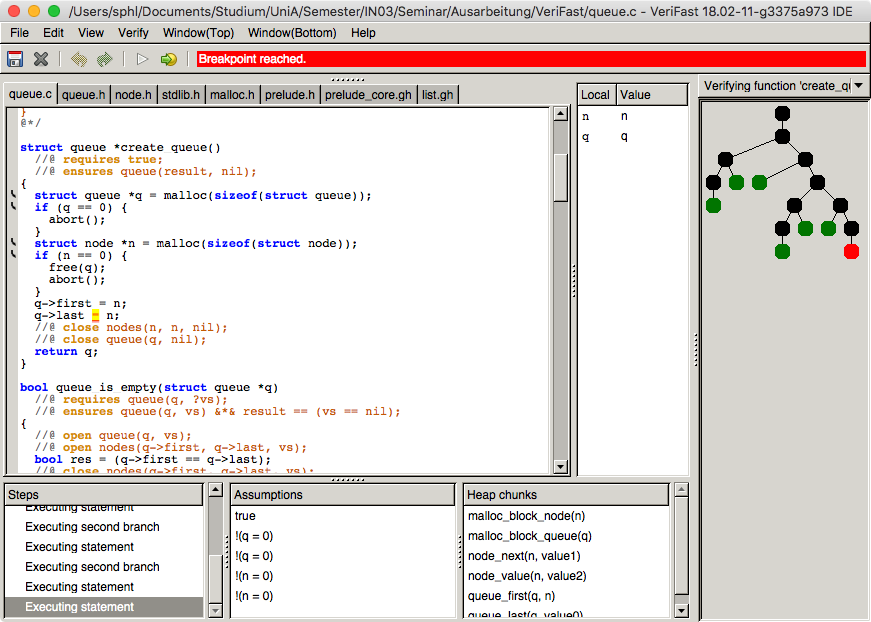
\includegraphics[width=0.8\linewidth]{verifast}
	\caption{VeriFast IDE}
	\label{fig:vfide}
\end{figure}

Während der Ausführung von VeriFast wird das Programm auf illegale Speicherzugriffe, beispielsweise durch Dereferenzierung von Null-Pointern oder durch Zugriff auf Speicherzellen außerhalb der Grenzen eines Arrays, sowie Fehler aufgrund nebenläufiger Ausführung (\emph{data races}) geprüft \cite{Jacobs2010}. Darüber hinaus verifiziert VeriFast die annotierten Methoden-Kontrakte - d.h. es wird versucht zu zeigen, dass sich die Nachbedingung aus der Vorbedingung und der symbolischen Ausführung des Methodenrumpfs ergibt. Diesbezüglich wird im Back-End Microsofts \emph{Z3} (\emph{SMT Solver}) verwendet.

Über die VeriFast IDE, die in \vref{fig:vfide} zu sehen ist, können Quellcodedateien editiert und Programme schrittweise oder in einem Durchlauf verifiziert werden. Im Falle eines Fehlers werden diese innerhalb des Editors lokalisiert und anhand einer Statusmeldung dem Benutzer mitgeteilt. Wurde die Verifikation erfolgreich durchlaufen, so können, abhängig von der ausgewählten Funktion, die durchlaufenen Pfade in Form eines Ausführungsbaums, der sich auf der rechten Seite der VeriFast IDE befindet, angezeigt werden. Zudem ermöglicht VeriFast über das Anklicken eines Blattknotens die Analyse einzelner Pfade. Die \emph{steps}-Auswahl in \cref{fig:vfide} listet hierbei die ausgeführten Schritte eines Pfades auf und erlaubt Sprünge zu vorherigen bzw. nachfolgenden Zuständen. Nebenan befinden sich die logischen Annahmen, die sich aus den Annotationen und dem ausgeführten C Code ergeben und somit die \emph{Pfadbedingung} $\Sigma$ bilden. Eine Besonderheit der IDE ist die Anzeige des \emph{symbolischen Heap} $h$, welcher abhängig vom Ausführungsschritt dessen Einträge (\emph{Heap Chunks}) darstellt. Darüber befindet sich der \emph{symbolische Store} $s$, welcher die Zuordnung der lokalen Variablen auf deren symbolischen Werte verwaltet. Dementsprechend ist der Pfadzustand durch das Tupel $(\Sigma, h, s)$ gegeben \cite{Jacobs2011}.

\subsection{Symbolischer Heap-Speicher}
\label{subsuc:malloc}

Charakteristisch für C ist die dynamische Speicherverwaltung mittels den beiden Funktionen \texttt{malloc} und \texttt{free}. Dadurch kann eine festgelegte Anzahl an Bytes angefordert und darauf, falls erfolgreich vom Betriebssystem alloziert, über einen Zeiger auf den Heap-Speicher zugegriffen werden. Da C über keine automatische \emph{Garbage Collection} (GC) verfügt, steht der Programmierer in der Pflicht, den Speicherbereich, falls dieser nicht mehr benötigt wird, manuell mit Hilfe von \texttt{free} zu räumen. Dementsprechend gilt es auch den Zustand des Heap-Speichers bei der Verifikation von Programmen zu berücksichtigen. Hierbei legt VeriFast sogenannte \emph{Chunks} auf dem symbolischen Heap-Speicher ab, wann immer eine Datenstruktur während der symbolischen Ausführung alloziert wird. Instanzen die über \texttt{malloc} erzeugt wurden, werden von VeriFast besonders behandelt. Diese erhalten neben dem normalen Heap-Eintrag einen zusätzlichen \texttt{malloc\_block} Chunk, welcher signalisiert das es sich um einen dynamischen Speicherblock handelt \cite{Jacobs2008,Jacobs2010}. Über diesen Mechanismus kann vor der Freigabe überprüft werden, ob die zu löschende Instanz über einen gültigen \texttt{malloc\_block} Eintrag verfügt. Ist dies der Fall, so kann der Speicherblock aus dem Heap-Speicher entfernt werden.

Das nachfolgende Listing zeigt die beiden C-Strukturen \texttt{node} und \texttt{queue}. Erstere stellt einen Knoten in einer einfach verketteten Liste dar, welche neben einer Variablen vom Typ \texttt{char}, einen Zeiger auf das nächste Listenelement enthält. \texttt{queue} verfügt über zwei Zeiger, die jeweils auf das erste bzw. letzte Element einer Warteschlange zeigen. Darüber hinaus ist die Funktion \texttt{create\_queue} zu sehen, welche Heap-Speicher für eine neue Queue alloziert und anschließend den Variablen \texttt{first} und \texttt{last} initial den gleichen Knoten zuweist. Die darin enthaltenen VeriFast-spezifischen Annotationen werden jedoch erst in \cref{subsec:vflang} erklärt und können somit an dieser Stelle vorerst übersprungen werden.

\vspace{-10pt}
{\noindent
\begin{minipage}[t]{.45\textwidth}
\begin{lstlisting}
struct node {
  struct node *next;
  char value;
};
\end{lstlisting}
\end{minipage}
\hfill
\begin{minipage}[t]{.45\textwidth}
\begin{lstlisting}
struct queue {
  struct node *first;
  struct node *last;
};
\end{lstlisting}
\end{minipage}
}

\begin{lstlisting}
struct queue *create_queue()
  //@ requires true;
  //@ ensures queue(result, nil);
{
  struct queue *q = malloc(sizeof(struct queue));
  if (q == 0) { abort(); }
  struct node *n = malloc(sizeof(struct node));
  if (n == 0) { abort(); }
  q->first = n;
  q->last = n;
  //@ close nodes(n, n, nil);
  //@ close queue(q, nil);
  return q;
}
\end{lstlisting}

\noindent
\cref{tab:heap-chunks} zeigt einen Ausschnitt des symbolischen Heap-Speichers während der Ausführung von \texttt{create\_queue}. Dabei stehen die symbolischen Werte \texttt{value1} und \texttt{value2} für beliebige Werte, da keine konkrete Zuweisung für die Variablen \texttt{next} und \texttt{value} des Knotens \texttt{n} vorgenommen wurde.

{\setlength\extrarowheight{3pt} % Vergroeßert den Zeilenabstand
\begin{table}[hbt!]
%	\centering
	\caption{Heap-Chunks}
	\begin{tabularx}{\textwidth}{|p{4.5cm}|X|}
		\hline
		\rowcolor{LightGrey1}
		%-----------------------------------------------------------------------------------------------------
		\textbf{Chunk}                   & \textbf{Beschreibung}                                     \\ \hline
		%-----------------------------------------------------------------------------------------------------
		\texttt{malloc\_block\_node(n)}  & Dynamisch allozierte Instanz \texttt{n}                   \\ \hline
		\texttt{malloc\_block\_queue(q)} & Dynamisch allozierte Instanz \texttt{q}                   \\ \hline
		\texttt{n->next |-> value1}      & Feld \texttt{next} hat symbolischen Wert \texttt{value1}  \\ \hline
		\texttt{n->value |-> value2}     & Feld \texttt{value} hat symbolischen Wert \texttt{value2} \\ \hline
		\texttt{q->first |-> n}          & Feld \texttt{first} zeigt auf Instanz \texttt{n}          \\ \hline
		\texttt{q->last |-> n}           & Feld \texttt{last} zeigt auf Instanz \texttt{n}           \\ \hline
		%-----------------------------------------------------------------------------------------------------
	\end{tabularx}
	\label{tab:heap-chunks}
\end{table}
}

\subsection{Konzepte der Verifikation}
\label{subsec:vflang}

In diesem Abschnitt werden einige Konzepte vorgestellt, die VeriFast für die Programmverifikation bereitstellt. Dabei werden vorzugsweise die Konzepte behandelt, welche für das Verständnis des Beispiels in \cref{subsec:queue} relevant sind. Weiterführende Konzepte und Beispiele können in \cite{Jacobs2017} nachgelesen werden.

\subsubsection{Kontrakte}

Kontrakte beschreiben einen Vertrag zwischen dem Aufrufer einer Methode und deren Implementierung. Dabei besitzt jede Methodendeklaration eine Vor- und Nachbedingung, die angeben, dass wenn die Vorbedingung (vom Aufrufer) erfüllt wird, die Nachbedingung von der Implementierung der Methode zugesichert werden kann. Zuvor gilt es allerdings für jeden Kontrakt zu zeigen, dass die Nachbedingung aus der Vorbedingung und dem finalen Pfadzustand folgt. Dieser Ansatz, der als \emph{Design-by-Contract} bezeichnet wird, wird auch von VeriFast verwendet, um die Korrektheit von C-Funktionen nachzuweisen. Für die Vor- und Nachbedingung stehen die Annotationen \texttt{requires} und \texttt{ensures} zur Verfügung, deren Bedingung in Form einer Formel definiert wird. Diese setzt sich wiederum aus Heap-Chunks und booleschen Ausdrücken zusammen, welche mittels \emph{Separation Conjunction} $(\&{*}\&)$ (Bestandteil der \emph{Separation Logic}) kombiniert werden.

Allgemein beschreibt Separation Logic eine Erweiterung der \emph{Hoare Logic}, welche Schlussfolgerungen über geteilte, änderbare Datenstrukturen, wie bspw. der Heap-Speicher in Java und C, erlaubt \cite{Reynolds2002}. Die Konjunktion $C_{1} \; \&{*}\& \; C_{2}$ beschreibt dabei, dass $C_{1}$ und $C_{2}$ auf disjunkten Speicherbereichen gelten und somit Änderungen keinen Einfluss bzw. Nebeneffekte auf andere Bereiche des Speichers haben.

Um zu zeigen das die Vorbedingung bei einem Methodenaufruf erfüllt wird, versucht VeriFast die in \texttt{requires} hinterlegte Formel zu \emph{konsumieren}. D.h. die enthaltenen Chunks und logischen Ausdrücke werden vom symbolischen Heap bzw. aus der Liste der Pfadannahmen entfernt. Ist dies nicht möglich, da bspw. ein zu konsumierender Chunk auf dem Heap nicht vorhanden ist, so schlägt die Verifikation fehl. Konnte hingegen die Vorbedingung gezeigt werden, so \emph{produziert} VeriFast neue Einträge für die in \texttt{ensures} enthaltene Formel \cite{Jacobs2017}. Dieser Vorgang hat den Vorteil, dass bei einem Unteraufruf nicht der komplette Methodenrumpf durchlaufen werden muss, sondern VeriFast lediglich die spezifizierte Formel konsumiert und produziert.

\subsubsection{Induktive Datentypen}
\label{subsubsec:adt}

Ein wichtiges Hilfsmittel um die Korrektheit von Programme nachzuweisen, besteht in der Spezifikation von abstrakten Datentypen (ADT). Diese ermöglichen es, Eigenschaften und Operationen eines Datentyps auf einem höheren Abstraktionsniveau, d.h. unabhängig von der konkreten Implementierung auf einem Computer, zu betrachten \cite[S. 265]{Saake2014}. Daraus resultierend, können ADTs in der Programmverifikation als Repräsentanten für die Inhalte konkrete Datenstrukturen, wie beispielsweise Arrays oder einfach- oder doppelt-verkettete Listen, eingesetzt werden.

VeriFast unterstützt den Einsatz von induktiven Datentypen, deren Instanzen über \emph{Konstruktorterme} gebildet werden. Die Spezifikation einer abstrakten Liste sieht dabei wie folgt aus.

\begin{lstlisting}
inductive list<t> = nil | cons(t, list<t>);
\end{lstlisting}

\noindent
In diesem Beispiel wurde eine generische Liste mit den Konstruktoren \texttt{nil} für die leere Liste und \texttt{cons} für die zusammengesetzte Liste, mit Kopfelement vom Typ \texttt{t} und Restliste des Datentyps \texttt{list<t>}, definiert. Analog zu den meisten Programmiersprachen, spezifiziert \texttt{<t>} den generischen Datentyp, wodurch Listen über \texttt{int}, \texttt{char}, \texttt{bool} etc. konstruiert werden können. So entspricht der Konstruktorterm \texttt{cons('a', cons('b', cons('c', nil)))} einer Liste mit der Zeichenfolge \texttt{<'a', 'b', 'c'>}.

\subsubsection{Fixpunkt Funktionen}

Neben den induktiven ADTs unterstützt VeriFast die Spezifikation von Fixpunkt Funktionen, wodurch spezifische Operation auf induktive Datentypen definiert werden können. Diese werden mit \texttt{fixpoint} eingeleitet und erhalten über die Parameterliste einen oder mehrere ADTs. Im Funktionsrumpf kann entweder direkt eine \texttt{return}-Anweisung, welche die berechnete Eigenschaft an den Aufrufer zurückgibt, oder eine \texttt{switch}-Anweisung stehen. Letztere führt eine Fallunterscheidung bezüglich aller Konstruktoren von genau einem induktiven Argument aus. Zudem prüft VeriFast jede Funktion auf Terminierung - d.h. im Falle eines rekursiven Aufrufs muss der Konstruktorterm des neuen Übergabeparameters ein Teilterm des alten Parameters sein \cite{Jacobs2010}.

Ausgehend von der induktiven Liste in \cref{subsubsec:adt}, definieren wir die beiden Funktionen \texttt{head} und \texttt{tail}, welche das Kopfelement bzw. die Restliste von \texttt{xs} zurückliefern.

\begin{lstlisting}
fixpoint t head<t>(list<t> xs) {
  switch (xs) {
    case nil: return default_value<t>;
    case cons(x, xs0): return x;
  }
}
fixpoint list<t> tail<t>(list<t> xs) {
  switch (xs) {
    case nil: return nil;
    case cons(x, xs0): return xs0;
  }
}
\end{lstlisting}

\noindent
Für den Konstruktor \texttt{cons(t, list<t>)} bindet VeriFast die entsprechenden Werte an die Variablen \texttt{x} und \texttt{xs0}, welche im Anschluss beliebig weiterverwendet werden können. Ein Sonderfall in diesem Beispiel ist der Konstruktor \texttt{nil} in \texttt{head}. Hierbei wird ein Defaultwert zurückgegeben, der je nach Anforderung und Datentyp unterschiedliche Werte annehmen kann.

Eine weitere bekannte Funktion auf Container-Datentypen ist \texttt{length}, welche in diesem Beispiel die Länge einer Liste rekursiv berechnet. Wurde ein Term ungleich \texttt{nil} übergeben, so wird dieser sukzessive abgebaut und zugleich die Länge um den Wert 1 erhöht. Der letzte Aufruf endet immer im \texttt{nil}-Konstruktor, welcher folgerichtig die Länge 0 zurückgibt und damit die Berechnung abschließt.%\footnote{Die Funktionen \texttt{head}, \texttt{tail}, \texttt{length} und weitere Fixpunkt-Operationen auf \texttt{list<t>} sind Bestandteil der VeriFast-Bibliothek.}

\begin{lstlisting}
fixpoint int length<t>(list<t> xs) {
  switch (xs) {
    case nil: return 0;
    case cons(x, xs0): return 1 + length(xs0);
  }
}
\end{lstlisting}

\subsubsection{Prädikate}

Prädikate werden dazu eingesetzt, um Aussagen, die wiederkehrend in unterschiedlichen Methodenkontrakten Verwendung finden, zu kapseln. Über den \texttt{close}-Befehl werden diese durch ein passendes Prädikat gebündelt, wobei die enthaltenen Chunks durch das entsprechende Prädikat auf dem Heap ersetzt werden. Die entgegengesetzte Wirkung erzielt \texttt{open}, dass ein Prädikat in dessen ursprüngliche Aussagen zerlegt \cite{Jacobs2008,Jacobs2017}.

%\begin{figure}[t]
%	\centering
%	\begin{minipage}{.45\textwidth}
%		\centering
%		\begin{tikzpicture}[scale=5.5]
	\draw [thick, white] (0.05,0.65) rectangle (1.0,0.0);
	\draw [thick, black, pattern color=LightGrey3, pattern=north east lines] (0.35,0.05) rectangle (0.95,0.45);
	% First row
	\draw [fill=LightGrey1] (0.1,0.1) rectangle (0.3,0.2) node[pos=.5] {$C_{7}$};
	\draw [fill=LightGrey1] (0.1,0.3) rectangle (0.3,0.4) node[pos=.5] {$C_{4}$};
	\draw [fill=LightGrey1] (0.1,0.5) rectangle (0.3,0.6) node[pos=.5] {$C_{1}$};
	% Second row
	\draw [fill=LightGrey1] (0.4,0.1) rectangle (0.6,0.2) node[pos=.5] {$C_{8}$};
	\draw [fill=LightGrey1] (0.4,0.3) rectangle (0.6,0.4) node[pos=.5] {$C_{5}$};
	\draw [fill=LightGrey1] (0.4,0.5) rectangle (0.6,0.6) node[pos=.5] {$C_{2}$};
	% Third row
	\draw [fill=LightGrey1] (0.7,0.1) rectangle (0.9,0.2) node[pos=.5] {$C_{9}$};
	\draw [fill=LightGrey1] (0.7,0.3) rectangle (0.9,0.4) node[pos=.5] {$C_{6}$};
	\draw [fill=LightGrey1] (0.7,0.5) rectangle (0.9,0.6) node[pos=.5] {$C_{3}$};
\end{tikzpicture}
%		\captionof{figure}{Prädikat \texttt{nodes}}
%		\label{fig:nodes}
%	\end{minipage}
%	\hfill
%	\begin{minipage}{.45\textwidth}
%		\centering
%		\begin{tikzpicture}[scale=5.5]
	\draw [thick, black, pattern color=LightGrey2, pattern=crosshatch dots] (0.05,0.5) rectangle (1.0,0.0);
	\draw [thick, black, preaction={fill, white},pattern color=LightGrey3, pattern=north east lines] (0.35,0.05) rectangle (0.95,0.45);
	% First row
	\draw [fill=LightGrey1] (0.1,0.1) rectangle (0.3,0.2) node[pos=.5] {$C_{2}$};
	\draw [fill=LightGrey1] (0.1,0.3) rectangle (0.3,0.4) node[pos=.5] {$C_{1}$};
	% Second row
	\draw [fill=LightGrey1] (0.4,0.1) rectangle (0.6,0.2) node[pos=.5] {$C_{4}$};
	\draw [fill=LightGrey1] (0.4,0.3) rectangle (0.6,0.4) node[pos=.5] {$C_{3}$};
	% Third row
	\draw [fill=LightGrey1] (0.7,0.1) rectangle (0.9,0.2) node[pos=.5] {$C_{6}$};
	\draw [fill=LightGrey1] (0.7,0.3) rectangle (0.9,0.4) node[pos=.5] {$C_{5}$};
\end{tikzpicture}
%		\captionof{figure}{Prädikat \texttt{queue}}
%		\label{fig:queue}
%	\end{minipage}
%\end{figure}

Das nachfolgende Listing zeigt die Prädikate \texttt{nodes} und \texttt{queue}, die in den beiden \texttt{close}-Anweisungen der Funktion \texttt{create\_queue} aus \cref{subsuc:malloc} verwendet wurden.

\vspace{-10pt}
{\noindent
\begin{minipage}[t]{.45\textwidth}
\begin{lstlisting}
predicate nodes(
    struct node *first,
    struct node *last,
    list<char> vs) =
  first == last ?
    vs == nil
  :
    first->next |-> ?next &*&
    first->value |-> ?val &*&
    malloc_block_node(first) &*&
    nodes(next, last, ?vs0) &*&
    vs == cons(val, vs0);
\end{lstlisting}
\end{minipage}
\hfill
\begin{minipage}[t]{.45\textwidth}
\begin{lstlisting}
predicate queue(
    struct queue *q,
    list<char> vs) =
  q->first |-> ?first &*&
  q->last |-> ?last &*&
  malloc_block_queue(q) &*&
  nodes(first, last, vs) &*&
  last->next |-> _ &*&
  last->value |-> _ &*&
  malloc_block_node(last);
\end{lstlisting}
\end{minipage}
}

\noindent
Innerhalb des Listings werde neue Variablen mittels \texttt{?var} eingeführt. Der symbolische Wert wird dabei an den Variablennamen gebunden, um explizite Aussagen über Variablenwerte formulieren zu können. Anders verhält es sich mit \texttt{\_}, dass als namenloser Platzhalter für beliebige Werte von VeriFast interpretiert wird \cite{Jacobs2017}. \texttt{nodes} beschreibt in diesem Beispiel ein rekursives Prädikat, dessen induktive Liste \texttt{vs} den Inhalt zwischen den Knoten \texttt{first} und \texttt{last} repräsentiert. Hierbei setzt sich \texttt{vs} aus dem aktuellen Wert und der Restliste \texttt{vs0}, die sich wiederum aus einem bereits vorhandenen \texttt{nodes}-Prädikat ergibt, zusammen.

Die Bedingung in \texttt{nodes} prüft zudem, ob \texttt{first} gleicht dem Knoten \texttt{last} ist. In diesem Fall existieren keine Zwischenknoten und \texttt{vs} gleicht einer leeren Liste. Hier gilt es zu beachten, dass \texttt{last} zu jeden Zeitpunkt auf einem Hilfsknoten zeigt, welcher keine Nutzdaten speichert. Das zweite Prädikat \texttt{queue} enthält neben \texttt{nodes} weitere Chunks und soll eine gültige Queue darstellen. %D.h. nach einer erfolgreichen Ausführung von \texttt{create\_queue} befindet sich \texttt{queue}, zusammen mit den entsprechenden Parametern, auf dem symbolischen Heap.

\subsubsection{Schleifeninvarianten}

Eine Schleifeninvariante (INV) ist ein Spezialfall einer Invariante. Diese beschreibt eine logische Aussage, die zu Beginn und Ende einer Schleife, sowie nach jedem Schleifendurchgang gelten bzw. erhalten bleiben muss. INV liefert somit eine Aussage über die Semantik des Schleifenrumpfs, die unabhängig von der Anzahl der Schleifendurchgänge gilt.

VeriFast zeigt für Schleifen ausschließlich \emph{partielle Korrektheit}\footnote{Anders als bei \emph{totaler Korrektheit} wird hierbei der Terminierungsnachweis ausgelassen.}, deren Verifikation wie folgt abläuft: \cite{Jacobs2017}

\begin{itemize}
	\item Zeige das INV vor dem ersten Durchlauf gilt (INV konsumieren)
	\item Zeige das INV nach jedem Durchlauf erhalten bleibt:
	\begin{enumerate}
		\item Symbolischen Heap temporär räumen und für jede lokale Variable innerhalb des Schleifenrumpfs ein \emph{frisches} Symbol vergeben
		\item INV erneut auf den symbolischen Heap legen (INV produzieren)
		\item Fallunterscheidung bzgl. der Schleifenbedingung: % $\epsilon$:
		\begin{itemize}
			% Vergroeßere den Abstand zwischen zwei Items, um diese besser lesbar zu machen
			\setlength\itemsep{3pt}
%			\item $[\![\epsilon]\!] = true:$
			\item Schleifenbedingung erfüllt:
			\begin{enumerate}
				\item Schleifenrumpf verifizieren und anschließend INV konsumieren
				\item Überprüfung weiterer \emph{Leaks} und Abschluss des Pfades
			\end{enumerate}
			\item Sonst, Heap zurücksetzen und mit der Verifikation des Folgeprogramms fortfahren
		\end{itemize}
	\end{enumerate}
\end{itemize}

\noindent
Ein Anwendungsfall einer Schleifeninvariante ist in \texttt{queue\_destroy} zu finden. Darin wird über all die Knoten in der Queue iteriert, welche die tatsächlichen Nutzdaten speichern, um diese nacheinander freizugeben. Demzufolge muss der letzte Hilfsknoten (\texttt{last}) außerhalb der Schleife gelöscht werden. Über die Schleifeninvariante gilt es zu zeigen, dass vor der Schleife und nach jedem Schleifendurchlauf das \texttt{nodes}-Prädikat, zusammen mit der passenden Listen-Abstraktion, konsumiert werden kann. 

\begin{lstlisting}
void queue_destroy(struct queue *q)
  //@ requires queue(q, _);
  //@ ensures true;
{
  //@ open queue(q, _);
  struct node *l = q->last;
  struct node *n = q->first;
  while (n != l)
    //@ invariant nodes(n, l, ?vs);
  {
    //@ open nodes(n, l, _);
    struct node *tmp = n->next;
    free(n);
    n = tmp;
  }
  //@ open nodes(n, l, _);
  free(l);
  free(q);
}
\end{lstlisting}

\subsubsection{Lemma Funktionen}
\label{subsubsec:lemma}

Lemma und C-Funktionen sind einander sehr ähnlich, da beide zuerst die Vorbedingung konsumieren und anschließend die Nachbedingung produzieren. Der Unterschied liegt darin, dass weder Variablenzuweisungen noch Methodenaufrufe enthalten sein dürfen. Des weiteren muss sichergestellt werden, dass rekursive Lemma Funktion in allen Pfaden terminieren. Welche Arten von Rekursion hierbei zulässig sind, wird in \cite[S. 22]{Jacobs2017} ausführlich beschrieben. Ziel einer solchen Funktion ist die Transformation einer Darstellung von Heap-Chunks in eine andere, wobei die zugrunde liegenden Chunks unverändert bleiben \cite{Jacobs2010}.

In Voraussicht auf die Funktion \texttt{queue\_enqueue} in \cref{subsec:queue}, soll an dieser Stelle die Lemma Funktion \texttt{nodes\_add} eingeführt werden.

\begin{lstlisting}
lemma void nodes_add(struct node *first)
  requires nodes(first, ?last, ?vs) &*&
    last->next |-> ?newLast &*&
    last->value |-> ?val &*&
    malloc_block_node(last) &*&
    newLast->next |-> ?nextNext;
  ensures nodes(first, newLast, ?vs0) &*&
    vs0 == append(vs, cons(val, nil)) &*&
    newLast->next |-> nextNext;
{
  open nodes(first, last, vs);
  if (first == last) {
      close nodes(newLast, newLast, nil);
  } else {
      nodes_add(first->next);
  }
  close nodes(first, newLast, _);
}
\end{lstlisting}

\noindent
Hier fordert \texttt{requires} eine gültige \texttt{nodes}-Abstraktion, in der \texttt{last} einen Folgeknoten besitzt. Dies bedeutet, die Queue wurde um einen Knoten erweitert, welcher noch nicht in der Abstraktion enthalten ist. Hierfür wird \texttt{nodes} innerhalb der Implementierung rekursiv aufgespalten, um anschließend das Prädikat sukzessive mit dem neuen Element zusammenzusetzen.

\subsection{Verifikation einer Queue}
\label{subsec:queue}

Im Verlauf dieser Sektion werden die Funktionen \texttt{queue\_enqueue} und \texttt{queue\_dequeue} beschrieben, mit deren Hilfe ein neues Element am Ende der Queue eingereiht bzw. das erste und älteste Element herausgenommen werden kann. Darüber hinaus wird die Schnittstellenfunktion \texttt{queue\_contains} vorgestellt, welche prüft, ob ein gesuchtes Element innerhalb der Queue enthalten ist.

\begin{figure}[t]
	\centering
	\newcommand{\chainlabel}[2]{\path [<-, draw, shorten >=17pt] (#1) |- node [at end] {#2} ++(-1,1);}

\begin{tikzpicture}[list/.style={rectangle split, rectangle split parts=2, draw, rectangle split horizontal}, >=stealth, start chain]
	\node[list,on chain] (A) {$c_{0}$};
	\node[list,on chain] (B) {$c_{1},\ldots,c_{n-1}$};
	\node[list,on chain] (C) {$c_{n}$};
	\node[list,on chain] (D) {};
	\node[on chain,draw,inner sep=6pt] (E) {};
	\draw (E.north east) -- (E.south west);
	\draw (E.north west) -- (E.south east);
	\draw[*->] let \p1 = (A.two), \p2 = (A.center) in (\x1,\y2) -- (B);
	\draw[*->] let \p1 = (B.two), \p2 = (B.center) in (\x1,\y2) -- (C);
	\draw[*->] let \p1 = (C.two), \p2 = (C.center) in (\x1,\y2) -- (D);
	\draw[*->] let \p1 = (D.two), \p2 = (D.center) in (\x1,\y2) -- (E);
	\chainlabel{chain-1.one north}{$\mathit{first}$};
	\chainlabel{chain-3.one north}{$last_{old}$};
	\chainlabel{chain-4.one north}{$last_{new}$};
	\draw[decoration={brace,mirror,raise=20pt},decorate]
	(A.west) -- node[below=25pt] {$nodes(\mathit{first}, \; last_{old}, \; vs)$} (B.east);
	\draw[decoration={brace,mirror,raise=50pt},decorate]
	(A.west) -- node[below=55pt] {$nodes(\mathit{first}, \; last_{new}, \; append(vs, \; cons(c_{n}, \; nil)))$} (C.east);
\end{tikzpicture}
	\caption{Ablauf von \texttt{queue\_enqueue}}
	\label{fig:list}
\end{figure}

\cref{fig:list} veranschaulicht den Zustand der Queue vor und nach der Ausführung von \texttt{queue\_enqueue}. Darin wird das Element $c_{n}$ eingefügt und anschließend \texttt{last} auf den neuen Hilfsknoten $last_{new}$ gesetzt. Innerhalb von \texttt{queue\_enqueue} kann nun die im vorherigen Abschnitt eingeführte Lemma Funktion \texttt{nodes\_add} eingesetzt werden, wodurch \texttt{nodes} den Inhalt der erweiterten Queue abstrahiert.

Die Schnittstellenfunktion \texttt{queue\_dequeue} benötigt hingegen keine zusätzliche Lemma Funktion, da \texttt{nodes(first, last, cons(val, vs))} genau einmal aufgespalten werden muss, um an das geschachtelte Folgeprädikat \texttt{nodes(first->next, last, vs)} zu gelangen. Dieses kann dann im nächsten Schritt erneut an \texttt{queue} gebunden werden, wodurch die Nachbedingung des Kontrakts erfüllt wird.

\vspace{-10pt}
{\noindent
\begin{minipage}[t]{.45\textwidth}
\begin{lstlisting}
void queue_enqueue(
    struct queue *q,
    char c)
  //@ requires queue(q, ?vs);
  /*@ ensures queue(q, append(vs,
        cons(c, nil))); @*/
{
  //@ open queue(q, vs);
  struct node *n =
    malloc(sizeof(struct node));
  if (n == 0) {
    abort();
  }
  q->last->next = n;
  q->last->value = c;
  q->last = n;
  //@ nodes_add(q->first);
  //@ close queue(q, _);
}
\end{lstlisting}
\end{minipage}
\hfill
\begin{minipage}[t]{.45\textwidth}
\begin{lstlisting}
char queue_dequeue(
    struct queue *q)
  /*@ requires queue(q, ?vs) &*&
        vs != nil; @*/
  /*@ ensures queue(q, ?vs0) &*&
        vs == cons(result, vs0); @*/
{
  //@ open queue(q, _);
  struct node *n = q->first;
  //@ open nodes(n, _, _);
  char result = n->value;
  q->first = n->next;
  free(n);
  //@ close queue(q, _);
  return result;
}
\end{lstlisting}
\end{minipage}
}

\noindent
Die Überprüfung, ob ein Element in der Queue enthalten ist, wird durch die Funktion \texttt{queue\_contains} realisiert. Die eigentliche Implementierung wurde jedoch nach \texttt{nodes\_contains} ausgelagert, um ausgehend vom Startknoten, alle weiteren Knoten rekursiv überprüfen zu können. Dabei wird der Inhalt des Startknotens mit dem gesuchten Element verglichen, dass Ergebnis in einer Variablen zwischengespeichert und anschließend die Funktion erneut mit dem Nachfolger des Startknotens aufgerufen.

Das Abbruchkriterium ist dann erfüllt, wenn Start- und Endknoten derselbe sind und somit die komplette Queue durchlaufen wurde. Abschließend werde die rekursiv berechneten Teilergebnisse über ein logisches OR miteinander verknüpft, dessen boolescher Ausdruck in der letzten \texttt{return}-Anweisung genau dann zu \emph{wahr} auswertet, wenn der Inhalt von mindestens einem Teilknoten, dem des gesuchten Elements entspricht.

\vspace{-10pt}
{\noindent
\begin{minipage}[t]{.45\textwidth}
\begin{lstlisting}
bool nodes_contains(
    struct node *f,
    struct node *l,
    char c)
  //@ requires nodes(f, l, ?vs);
  /*@ ensures nodes(f, l, vs) &*&
        result == mem(c, vs); @*/
{
  //@ open nodes(f, l, vs);
  bool res = false;
  if (f != l) {
    bool cmp = (f->value == c);
    bool tmp = nodes_contains(
      f->next, l, c);
    res = (cmp || tmp);
  }
  //@ close nodes(f, l, vs);
  return res;
}
\end{lstlisting}
\end{minipage}
\hfill
\begin{minipage}[t]{.45\textwidth}
\begin{lstlisting}
bool queue_contains(
    struct queue *q,
    char c)
  //@ requires queue(q, ?vs);
  /*@ ensures queue(q, vs) &*&
        result == mem(c, vs); @*/
{
  //@ open queue(q, vs);
  bool res = nodes_contains(
    q->first, q->last, c);
  //@ close queue(q, vs);
  return res;
}
\end{lstlisting}
\end{minipage}
}

%\subsection{Praxis Fallstudien}

%\subsubsection{Embedded Linux Network Management Software}

%\subsubsection{Linux USB BP Keyboard Driver}

%\subsection{Fazit}
